\section{Synthetic Data Source Provenance}
\label{app:synth_prov}

To ensure full transparency regarding the "permissive-first" nature of \MixtureVitae{}, we provide a detailed provenance audit of our synthetic data components in Table~\ref{tab:provenance}, including classification to tiers as defined in Section~\ref{sec:license_tiers}.

\begin{table*}[htbp]
\vspace{-0.5cm}
\caption{Detailed provenance of synthetic data sources in \MixtureVitae{}.}

\centering
% Local tweaks so they don't affect other tables
\scriptsize
\setlength{\tabcolsep}{3pt}      % default is 6pt
\setlength{\extrarowheight}{0pt}
\renewcommand{\arraystretch}{0.99} % slightly more compact rows
\vspace{-0.2cm}

\begin{tabularx}{\textwidth}{
  >{\raggedright\arraybackslash}p{2.6cm}   % Dataset
  >{\centering\arraybackslash}p{1.3cm}     % Licensep3
  >{\centering\arraybackslash}p{1.0cm}     % Model
  >{\raggedright\arraybackslash}X          % Seed Data (flex)
  >{\centering\arraybackslash}p{0.9cm}     % Token Count
  >{\raggedright\arraybackslash}X          % Notes (flex)
}
\textbf{Dataset Name} & \textbf{\shortstack[r]{Dataset \\ License}} & \textbf{Model} & \textbf{\shortstack[r]{Seed Data \\ Provenance}} & \textbf{\shortstack[c]{Token\\Count(B)}} & \textbf{Notes} \\
\rowcolor{green!7} \multicolumn{6}{l}{\textbf{Tier 1: Fully Permissive ($\approx$ 161B Tokens)}} \\
\href{https://huggingface.co/datasets/glaiveai/reasoning-v1-20m}{GlaiveAI Reasoning} & Apache 2.0 & Permissive & N/A & 38.366 & Fully synthetic \\
\href{http://nvidia/Llama-Nemotron-Post-Training-Dataset}{Nemotron (Science \& Math)} & CC-BY-4.0 & Permissive & Permissive (StackOverflow, WildChat) & 22.310 & Science \& Math subset of Llama-Nemotron-Post-Training-Dataset \\
\href{https://huggingface.co/datasets/inclusionAI/Ling-Coder-SyntheticQA}{Ling-Coder/SyntheticQA} & Apache 2.0 & Permissive & N/A & 19.852 &  \\
\href{https://huggingface.co/datasets/open-thoughts/OpenThoughts3-1.2M}{Open Thoughts} & Apache 2.0 & Permissive & Permissive (OpenMath-2-Math, CodeGolf, OpenCode, etc) & 18.786 & Excludes Organic Chemistry subset \\
EuroPat & Public Domain & Permissive & Permissive & 11.586 & Synthetic image captions created from patents \\
\href{https://huggingface.co/datasets/Muennighoff/P3}{P3 (Permissive Subset)} & Apache 2.0 & N/A &
Permissive (ARC, PIQA, BoolQ, etc) &   10.130  & \\
\href{https://huggingface.co/datasets/nvidia/Nemotron-CC-v2}{Nemotron-CC} & Common Crawl ToS & Permissive & Permissive (Common Crawl) & 6.230 & Using a Permissive-only subset \\
YouTube & CC-BY-4.0 & Permissive & Permissive (VALID, CommonCorpus) & 7.386 & Derived from CC-BY licensed YouTube content \\
\href{https://huggingface.co/datasets/nvidia/Nemotron-PrismMath}{Prism-Math} & CC-BY-4.0 & Permissive & Permissive (NuminaMath-1.5) & 5.682 &  \\
\href{https://huggingface.co/datasets/deepmind/math_dataset}{DeepMind Math} & Apache 2.0 & N/A & Permissive (Procedurally Generated) & 4.232 &  \\
\href{https://huggingface.co/datasets/nvidia/OpenMathInstruct-1}{Misc. Instruct. / NVidia OpenMathInstruct-1} & NVIDIA license & Permissive & Permissive (GSM8K, MATH) & 2.440 &  \\
 \href{https://huggingface.co/datasets/HuggingFaceM4/WebSight}{Websights} & CC-BY-4.0 & Permissive & N/A & 1.018 & Fully synthetic \\
\href{https://huggingface.co/datasets/oumi-ai/MetaMathQA-R1}{Misc Instruct. / MetaMathQA-R1}
(responses) & MIT & Permissive & Permissive (GSM8K, MATH) & 0.672 &  \\
Math Word Problems & Apache 2.0 & N/A & Permissive & 0.456 & Procedurally Generated \\
\href{https://huggingface.co/datasets/inclusionAI/Ling-Coder-DPO}{Ling-Coder/DPO} & Apache 2.0 & Permissive & Unknown (Common-Crawl) & 0.398 &  \\
\href{https://huggingface.co/datasets/open-r1/OpenR1-Math-220k}{Misc. Instruct. / \newline  OpenR1-Math-220k} & Apache 2.0 & Permissive & Permissive (NuminaMath-1.5) & 0.320 &  \\
\href{https://huggingface.co/datasets/nvidia/sft_datablend_v1}{Misc. Instruct. / \newline  NVIDIA SFT Datablend} & CC-BY-4.0 & Permissive & Permissive (MNLI, COPA, PIQA, etc) & 0.286 &  \\
\href{https://huggingface.co/datasets/open-r1/OpenThoughts-114k-Code_decontaminated}{Misc. Instruct. / \newline  OpenThoughts-114k-Code (decontaminated)} & Apache 2.0 & Permissive & Permissive (TACO, Apps , CodeContests, etc) & 0.150 &  \\
\href{https://huggingface.co/datasets/VishaalY/synthetic-code-generations}{Misc. Instruct. / \newline Synthetic Code Generations} & Apache 2.0 & Permissive & N/A & 0.104 & Fully synthetic \\
\href{https://huggingface.co/datasets/PrimeIntellect/stackexchange-question-answering}{Misc. Instruct. / \newline  PrimeIntellect StackExchange QnA} & Apache 2.0 & N/A & N/A & 0.076 &  \\
\href{https://huggingface.co/datasets/PrimeIntellect/real-world-swe-problems}{Misc. Instruct. / \newline  PrimeIntellect Real World SWE Problems} & Apache 2.0 & Permissive & Permissive (CommitPack) & 0.006 &  \\
\href{https://huggingface.co/datasets/PrimeIntellect/synthetic-code-understanding}{Misc. Instruct. / \newline  PrimeIntellect Synthetic Code Understanding} & Apache 2.0 & Permissive & N/A & 0.004 & Fully synthetic \\
\href{https://huggingface.co/datasets/openai/gsm8k}{Misc. Instruct. / \newline  GSM8K (train)} & MIT & Permissive & N/A & 0.004 & Fully synthetic \\
\rowcolor{yellow!10} \multicolumn{6}{l}{\textbf{Tier 2(a): Permissive with Upstream Opacity ($\approx$ 35B Tokens)}} \\
\href{https://huggingface.co/datasets/nvidia/OpenScience}{OS-Q2 (OpenScience)} & CC-BY-4.0 & Permissive & N/A & 17.366 & Fully synthetic \\
%\href{https://huggingface.co/datasets/Muennighoff/P3}{P3} & Apache 2.0 & N/A & Permissive (ARC, PIQA, BoolQ, etc) & 17.188 &  \\
\href{https://huggingface.co/datasets/inclusionAI/Ring-lite-sft-data}{Ring-lite SFT Data} & Apache 2.0 & Permissive & Permissive (CodeContest, APPS, TACO, etc) & 14.968 &  \\
\href{https://huggingface.co/datasets/hkust-nlp/CodeIO-PyEdu-Reasoning}{PyEdu Reasoning} & Stack V1, ODC-BY & Permissive & Permissive (The Stack V1) & 3.138 &  \\
\href{https://huggingface.co/datasets/Magpie-Align/Magpie-Phi3-Pro-1M-v0.1}{Misc. Instruct. / \newline  Magpie-Phi3-Pro-1M-v0.1} & N/A & Permissive & N/A & 0.386 & Fully synthetic \\
\href{https://huggingface.co/datasets/hltcoe/megawika}{MegaWika} & CC-By-SA/4.0 & Permissive & Permissive (Wikipedia) & 0.356 &  \\
\href{https://huggingface.co/datasets/Magpie-Align/Magpie-Qwen2.5-Coder-Pro-300K-v0.1}{Misc. Instruct. / \newline  Magpie-Qwen2.5-Coder-Pro-300K-v0.1} & N/A & Permissive & N/A & 0.120 & Fully synthetic \\
\href{https://huggingface.co/datasets/NovaSky-AI/Sky-T1_data_17k}{Misc. Instruct. / \newline  NovaSky-AI Sky-T1} & Apache 2.0 & Permissive & Permissive (AIME, MATH, etc) & 0.080 &  \\
\href{https://huggingface.co/datasets/bigcode/self-oss-instruct-sc2-exec-filter-50k}{Misc. Instruct. / \newline  BigCode Self-OSS-Instruct} & Stack v1 & Permissive & Permissive & 0.018 &  \\
\href{https://huggingface.co/datasets/openbmb/UltraFeedback}{Misc. Instruct. / \newline  UltraFeedback} & MIT & Permissive & Permissive (UltraChat, 
TruthfulQA, etc) & 0.014 &  \\
\href{https://huggingface.co/datasets/nguyenkhanh87/CaseHOLD_Phi4_Reasoning}{Misc. Instruct. / \newline  CaseHOLD (Phi4 Reasoning Traces)} & N/A & Permissive & Permissive (CaseHOLD) & 0.002 & Case law is public domain  \\
\rowcolor{orange!10} \multicolumn{6}{l}{\textbf{Tier 2(b): Restricted, Mixed or Opaque Provenance ($\approx$ 17B Tokens)}} \\
\href{https://huggingface.co/datasets/inclusionAI/Ling-Coder-SFT}{Ling-Coder/SFT} & Apache 2.0 & Permissive & Partially Unknown (Github, CommonCrawl, The Stack, etc) & 7.668 & Unknown provenance of CommonCrawl subset \\
P3 (Commercial Subset) & Apache 2.0  & N/A &
Ambiguous-license (Amazon, Rotten Tomatoes, IMDb, etc) & 5.730 &
User-generated content on commercial platforms with no verifiable licenses \\
\href{https://huggingface.co/datasets/nvidia/OpenMathInstruct-2}{Misc. Instruct. / \newline  OpenMathInstruct-2} & CC-By-4.0 & Restricted & Permissive (GSM8K and MATH) & 3.202 & Llama-generated responses \\
%\href{https://huggingface.co/datasets/oumi-ai/MetaMathQA-R1}{Misc. Instruct. / \newline MetaMathQA-R1}
%(questions) & MIT & Restricted & Permissive & 0.048 & ChatGPT-generated from permissive seeds \\
\href{https://huggingface.co/datasets/CharlieDreemur/OpenManus-RL}{Misc. Instruct. / \newline  OpenManus-RL} & Apache 2.0 & Mixed & Permissive (AgentTraj-L, Agent-FLAN, etc) & 0.024 & GPT-4 used for generating traces in the AgentTraj-L subset \\
\rowcolor{yellow!10} \multicolumn{6}{l}
{\textbf{Tier 3: Civic / Governmental Works ($\approx$ 15B Tokens)}} \\
\href{https://huggingface.co/datasets/nvidia/Nemotron-CC-v2}{Nemotron-CC (Gov. Portion)} & Common Crawl ToS & Permissive & Permissive (Common Crawl) & 8.531 & Using a Permissive-only subset \\
\href{https://huggingface.co/datasets/ByteDance-Seed/mga-fineweb-edu}{MGACorpus} & ODC-By & Permissive & Permissive (FinewebEdu-dedup) & 6.596 & Using only permissive subsets \\
\end{tabularx}
\label{tab:provenance}
\end{table*}


To validate the robustness of our permissive-first strategy, we further analyze the contribution of synthetic components categorized as \textbf{Tier 2(b)}. This small part of \MixtureVitae{} is comprised of subsets which are permissively licensed (e.g., Apache 2.0) but are derived from generator models with restrictive community licenses (such as Llama-3) or seed data with partially opaque origins. As illustrated in Figure~\ref{fig:ablate_tier2b}, removing these Tier 2(b) components yields a training trajectory indistinguishable from the full \MixtureVitae{} baseline. This result confirms that our model's strong performance is driven by its core, fully verifiable permissive sources, ensuring that users with strict compliance requirements can safely exclude Tier 2(b) data without compromising downstream quality.

See Section~\ref{app:govt_works} for a further discussion on our justification for including Tier 2 and in particular Tier 2(b) data.


\begin{figure}[htbp]
    \centering
        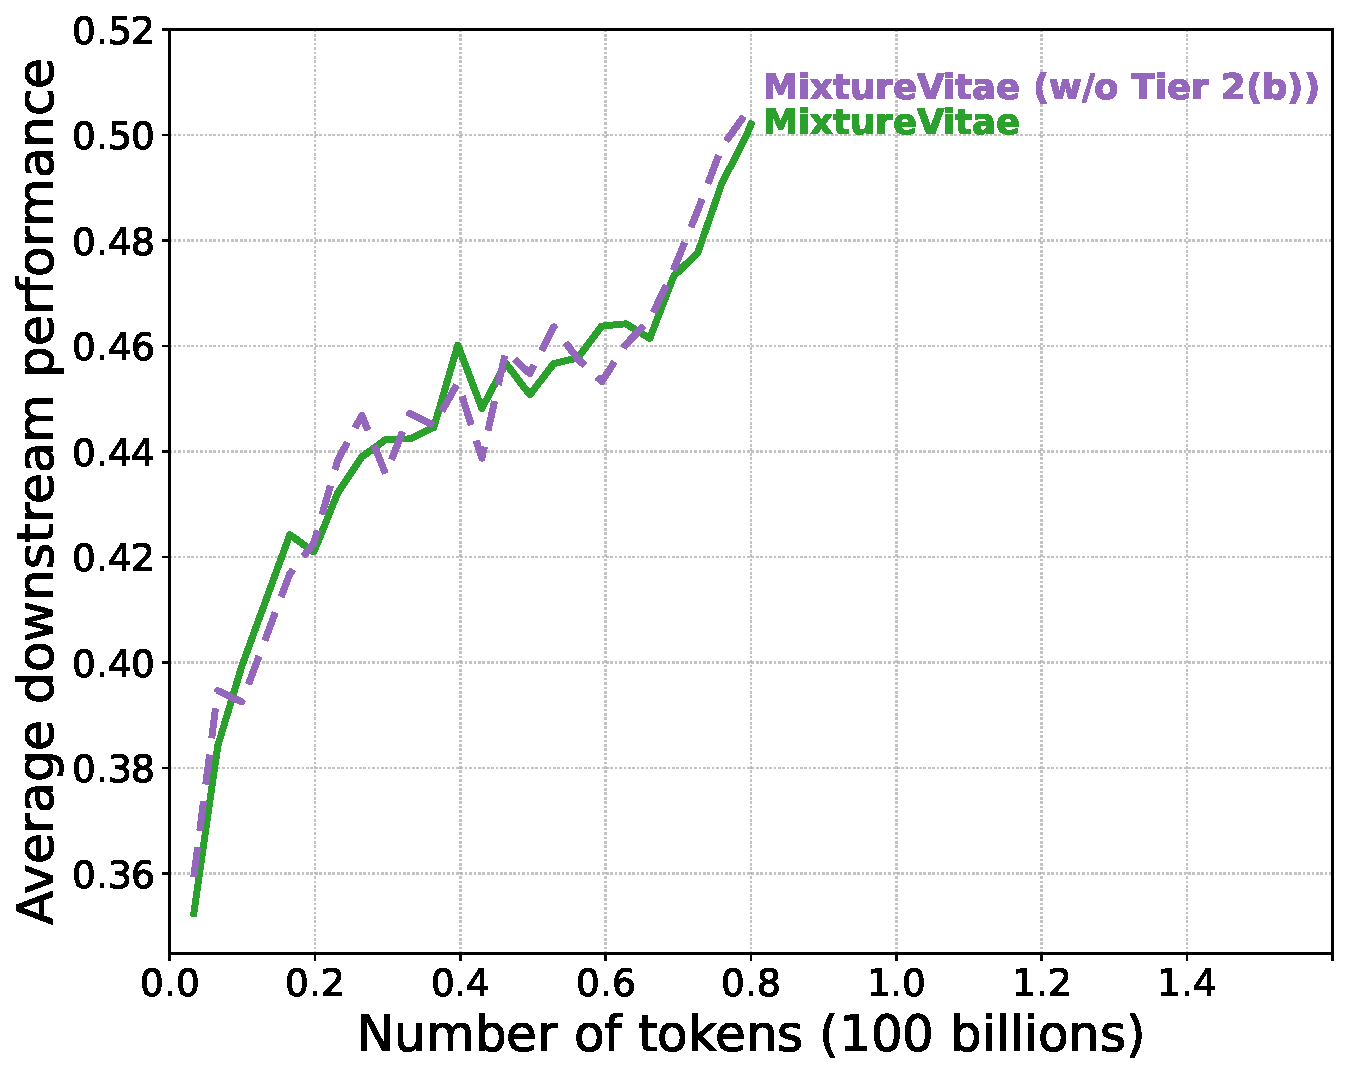
\includegraphics[width=0.48\linewidth]{figures/100B_perf_wo_tier2b.pdf}
        \caption{\textbf{Ablation of Tier 2(b) components.} We compare the training trajectory of the full \MixtureVitae{} dataset (green) against a version excluding Tier 2(b) (purple dashed). Tier 2(b) consists of synthetic data derived from non-permissive generators (e.g., Llama-3) or seeds with opaque provenance. The nearly identical performance curves demonstrate that users requiring strict permissive compliance can exclude these components with negligible impact on downstream model quality.}
        \label{fig:ablate_tier2b}
\end{figure}